
\documentclass[%
 reprint,
superscriptaddress,
%groupedaddress,
%unsortedaddress,
%runinaddress,
%frontmatterverbose,
%preprint,
%showpacs,preprintnumbers,
%nofootinbib,
%nobibnotes,
%bibnotes,
 amsmath,amssymb,
 aps,
%pra,
%prb,
%rmp,
%prstab,
%prstper,
%floatfix,
]{revtex4-1}

\usepackage{graphicx}% Include figure files
\usepackage{dcolumn}% Align table columns on decimal point
\usepackage{bm}% bold math
\usepackage{multirow}
\usepackage{threeparttable}
\hyphenpenalty=5000
\tolerance=1000
%\usepackage{hyperref}% add hypertext capabilities
%\usepackage[mathlines]{lineno}% Enable numbering of text and display math
%\linenumbers\relax % Commence numbering lines

%\usepackage[showframe,%Uncomment any one of the following lines to test
%%scale=0.7, marginratio={1:1, 2:3}, ignoreall,% default settings
%%text={7in,10in},centering,
%%margin=1.5in,
%%total={6.5in,8.75in}, top=1.2in, left=0.9in, includefoot,
%%height=10in,a5paper,hmargin={3cm,0.8in},
%]{geometry}

\begin{document}

\title{Study of the low-lying negative-parity states in $^{11}$Be  using the $^{12}$B($d$,$^{3}$He)$^{11}$Be reaction} % Force line breaks with \\
%\thanks{A footnote to the article title}%

\author{J.~Chen}
 \email{jie.chen@anl.gov}
\affiliation{Physics Division, Argonne National Laboratory, Argonne, Illinois 60439, USA}


\author{K. Auranen}
\affiliation{Physics Division, Argonne National Laboratory, Argonne, Illinois 60439, USA}

\author{M.~L.~Avila}
\affiliation{Physics Division, Argonne National Laboratory, Argonne, Illinois 60439, USA}

\author{B.~B.~Back}
\affiliation{Physics Division, Argonne National Laboratory, Argonne, Illinois 60439, USA}

\author{C.~R.~Hoffman}
\affiliation{Physics Division, Argonne National Laboratory, Argonne, Illinois 60439, USA}


\author{D.~Gorelov}
\affiliation{University of Manitoba, Department of Physics and Astronomy, Allen Building, Winnipeg, MB R3T 2N2, Canada}
\affiliation{Physics Division, Argonne National Laboratory, Argonne, Illinois 60439, USA}

\author{B.~P.~Kay}
\affiliation{Physics Division, Argonne National Laboratory, Argonne, Illinois 60439, USA}

\author{S.~A.~Kuvin}
\affiliation{Department of Physics, University of Connecticut, Storrs, Connecticut 06269, USA}
\affiliation{Physics Division, Argonne National Laboratory, Argonne, Illinois 60439, USA}
\author{Q.~Liu}%
\affiliation{%
 School of Physics and State Key Laboratory of Nuclear Physics and Technology, Peking University, Beijing 100871, China}%

\author{D.~G.~McNeel}
\affiliation{Department of Physics, University of Connecticut, Storrs, Connecticut 06269, USA}
\affiliation{Physics Division, Argonne National Laboratory, Argonne, Illinois 60439, USA}

\author{T.~L.~Tang}
\affiliation{Physics Division, Argonne National Laboratory, Argonne, Illinois 60439, USA}

\author{D.~Santiago-Gonzalez}
\affiliation{Physics Division, Argonne National Laboratory, Argonne, Illinois 60439, USA}

\author{J.~P.~Schiffer}
\affiliation{Physics Division, Argonne National Laboratory, Argonne, Illinois 60439, USA}

\author{R.~Talwar}
\affiliation{Physics Division, Argonne National Laboratory, Argonne, Illinois 60439, USA}


\author{J.~Wu}
\affiliation{Physics Division, Argonne National Laboratory, Argonne, Illinois 60439, USA}

\author{G.~Wilson}
\affiliation{Department of Physics and Astronomy, Louisiana State University, Baton Rouge, Louisiana 70803, USA}
\affiliation{Physics Division, Argonne National Laboratory, Argonne, Illinois 60439, USA}

\author{C.~X.~Yuan}
\affiliation{%
Sino-French Institute of Nuclear Engineering and Technology, Sun Yat-Sen University, Zhuhai 519082, China
}%


\author{H.~L.~Zang}%
\affiliation{%
 School of Physics and State Key Laboratory of Nuclear Physics and Technology, Peking University, Beijing 100871, China}%




\date{\today}

\begin{abstract}
The $p$-wave neutron configuration of the low-lying negative-parity states in $^{11}$Be were studied using the $^{12}$B($d,^3$He)$^{11}$Be reaction in inverse kinematics. The $1/2^-_1$ state at 0.32 MeV, the $3/2^-_1$ state at 2.56 MeV and one or both of the doublets including the $5/2^-_1$ state at 3.899 MeV and the $3/2^-_2$ state at 3.955 MeV were populated in the present reaction. Spectroscopic factors were determined from the cross sections using a distorted wave Born approximation method. The $0p_{3/2}$ proton removal strengths were well described by the shell model calculations using the YSOX interaction.%, while the Nilsson model calculation underestimated the strengths for higher excited states. Together with the $^{11}$B($d,^3$He)$^{10}$Be reaction data, the $0p_{1/2}$ neutron shows a weak coupling with the $^{10}$Be core in the $^{11}$Be low-lying negative-parity states.
\end{abstract}

\pacs{Valid PACS appear here}

\maketitle

\section{\label{sec:level1}Introduction}

%$^{11}$Be was extensively studied as a neutron-halo nucleus, which is usually interpreted as a $^{10}$Be core surrounded by a loosely bound valence neutron. Its small one-neutron separation energy of 502 keV~\cite{Wang_2017} together with the dominant $s$-wave configuration of the valence neutron lead to a very extended neutron-density distribution ~\cite{Tanihata,Schmitt}. The parity inversion of its ground state ($1/2^+$) was predicted by Talmi and Unna~\cite{Talmi} and confirmed by the experimental measurement of Alburger {\it et al.}~\cite{Alburger}. %The ground state of 11Be contains, in addition to the dominant 10Be(0+) + n(s1/2) configuration, a significant admixture (��20%) of core-excited components, with the valence neutron preferably occupying the d5/2 orbit [9�C11].
%It is noticed that around $Z=4$ and 5 the $s$ and $p$ orbital are inverted with respect to each other (see Fig.~1 of Ref.~\cite{Hoffman2014}). It is thus of great interest to study the evolution from $Z=5$ ($^{12}$B) to $Z=4$ ($^{11}$Be) via removal of one proton.

%It has been found that the binding energy plays a critical role in describing the variation in energy of $s$ states relative to other states~\cite{Hoffman2014}. Compared to $p$ or $d$ orbital, the linger behavior of $s$-wave neutrons near threshold resulted in the intrusion of the $1s_{1/2}$ orbital into the $0p$ shell. This effect is illustrated for a subset of the experimental information (nuclei with seven neutrons) in Fig.~1 of Ref.~\cite{Hoffman2014}.


%There have been several recent experiments to map out the level structure of $^{11}$Be. Hirayama {\it et al.}~\cite{HIRAYAMA2005}, Aoi {\it et al.}~\cite{AOI1997}, and Morrissey {\it et al.}~\cite{MORRISSEY1997} studied beta decay of $^{11}$Li, and excited state in $^{11}$Be including 1.778 MeV-($5/2^+$), 2.690 MeV-($3/2^-$), and 3.949 MeV-($3/2^-$) were observed~\cite{KELLEY2012}. The $^9$Be$(t,p)^{11}$Be reaction suggested assignment for the spins and parities of the low-lying states in $^{11}$Be and some of the states were indicated to be dominated by the two-neutron intruder configuration couple to $^9$Be g.s, including $3/2^-$ state at 3.955 MeV and $5/2^-$ state at 5.26 MeV~\cite{Liu1990}. The 3.89-MeV was assigned as $3/2^-$ based on the angular distribution, which was later questioned by Hirayama {\it et al.}~\cite{HIRAYAMA2005}. %Several neutron knockout reactions~\cite{Pain,Navin,Peters} demonstrated the importance of $sd$- intruder states to understanding the structure of $^{11}$Be, by populating the $1/2^+$ and $1/2^-$ states. % SF of resonances were analyzed using the calculated single-particle decay width comparing to the experimental widths.
%One of them~\cite{Peters} also claimed non-observation of the 3.887-MeV state in this measurement, which was later questioned by Fortune~\cite{Fortune2012}.

%More recently, there has been a $^{10}$Be$(d,p)$ transfer reaction~\cite{Schmitt} confirming the dominant single-particle $s$- and $p$-wave configuration in the g.s. and $1/2^-$. Inelastic scattering reaction on the carbon target populated low-lying resonances at 1.78 and 3.41 MeV, indicating they are $5/2^+$ and $3/2^+$ states. The later assignment does not agree with the $^9$Be$(t,p)$~\cite{Liu1990} reaction nor the $^{11}$Li beta-decay result~\cite{HIRAYAMA2005}.

%Two proton pickup reaction on $^{13}$C populated the member of the $1/2^-_1$ band of $^{11}$Be up to the $5/2^-$ state at 3.90 MeV~\cite{BOHLEN2003}. This band is believed to be headed with the relatively bound states ($1/2^-_1$) and terminated by the $7/2^-$ state, which is currently not well-known. The $2n$ transfer reaction on the well-developed $\alpha:n:\alpha$ structure in $^9$Be(g.s.) populated the molecular structure of $^{11}$Be and suggested a long rotational band $K^{\pi}=3/2^-$ build on the 3.96-MeV state~\cite{Bohlen2008}. The band was found to have a very larger moment of inertia than the $1/2^-_1$ band, which is an indication of the molecular structure.

In the light nuclei, the structure of the Be isotopes provides a great testing ground in some of the simplest nuclei for the approximations
made in the shell-model, the cluster model and the Nilsson model (where ``deformation" must arise from only the very few $p$-shell nucleons),  as well as the less model-dependent {\it ab-initio} calculations. The strong clustering in $^{8}$Be was evidenced by the ground state rotational band and the enhanced E2 transition. This naturally suggests that deformation degree of freedom will play an important role in the structure of the Be isotopes. In $^{11}$Be, this was confirmed by some indications for the rotational bands with $K^{\pi}=1/2^+,1/2^-$ and $3/2^-$~\cite{Bohlen2008,BOHLEN2003}.
  In a recent work by Macchiavelli {\it et al.}~\cite{Macchiavelli}, they interpreted the structure of Be isotopes within the Nilsson strong coupling limit and obtained good agreement with most available structure and reaction data. To fully complete the picture of Be isotopes, we study the  proton
spectroscopic factors of the $^{12}$B$(d,^3$He)$^{11}$Be reaction.
 The ground state of $^{11}$Be is usually interpreted as a halo state, with the $^{10}$Be core %surrounded by
inside a cloud of a loosely bound valence neutron. Based on this picture, $^{11}$Be low-lying states were also understood in the shell-model single-particle framework. The famous orbital inversion of $0p_{1/2}$ and $1s_{1/2}$ single-particle orbital was observed in $^{11}$Be compared to $N=7$ isotone $^{12}$B. Via proton removal from $^{12}$B, the evolution of the low-lying states from $^{12}$B to $^{11}$Be will be studied.

 The duality of the collective and single-particle descriptions of the atomic nucleus structure has been confirmed by recent experimental work~\cite{Santiago}, and the present system provides a unique testing ground for it. Further, the less model-dependent {\it ab-intio} calculations, which aspire to be able to predict rotational band structure in light nuclei, could be tested with descriptions of $^{11}$Be.

The low-lying negative-parity states have been studied using the $^9$Be$(t,p)^{11}$Be reaction~\cite{Liu1990} and $\beta$-decay of $^{11}$Li~\cite{HIRAYAMA2005,MORRISSEY1997,AOI1997}. These works understood structure of the low-lying negative-parity states in the shell-model framework. From the viewpoint of molecular structure, the negative-parity states with $\nu(2p-2h)$ configuration were understood to be the members of the molecular band with two alpha center~\cite{Bohlen2008}. The $^9$Be($^{13}$C,$^{11}$C)$^{11}$Be transfer reaction on the well-developed $\alpha:n:\alpha$ structure of $^9$Be(g.s.) populated the molecular structure of $^{11}$Be and suggested a long rotational band $K^{\pi}=3/2^-$ built on the 3.96-MeV $3/2^-$ state, which extends to $13/2^-$ state~\cite{BOHLEN2003}. Another band is believed to be headed with the relatively bound $1/2^-_1$ states and terminated by the $7/2^-$ state, which is currently not well studied.

 In the present work, we test various descriptions of $^{11}$Be using the $^{12}$B$(d,^3$He)$^{11}$Be reaction, including effective-interaction shell-model, Nilsson-model, VMC calculations and No-core shell-model calculations. Studies on $^{12}$B indicates the dominance of $p$-orbital neutron configuration~\cite{Mairle,Lind,LeeHY}.
 With removal of one $0p_{3/2}$ orbital proton, the negative parity state in $^{11}$Be are possibly populated. The $^{12}$B$(d,^3$He)$^{11}$Be reaction is a probe of the neutron $p$-wave strength in $^{11}$Be.
The present $^{12}$B$(d,^3$He)$^{11}$Be reaction solidities the low-lying negative-parity states and determines if there are any strengths within $p$-shell orbitals. Negative-parity states with large $\nu(2p-2h)$ configuration will not be strongly populated in this reaction, although allowed by the transferred angular momentum. An overall interpretation of the low-lying negative-parity states will be presented, which shed light on the mixing between $sd$- and $p$-shell as well as the structures of the $p$-shell states in $^{11}$Be.





\section{Experiment}

The $^{12}$B($d,^3$He)$^{11}$Be reaction was carried out in inverse kinematics, at the Argonne National Laboratory ATLAS In-Flight Facility. The 12 MeV/u $^{12}$B secondary beam was produced using the neutron adding reaction on a $^{11}$B primary beam at 13.5 MeV/u. This beam with an intensity of 200 pnA bombarded a 3.7-cm long D$_2$ gas cell at a pressure of 1400 mbar and temperature of 90 K. The resulting $^{12}$B was approximately $2\times10^5$ particle per second and had very little contamination (less than $5\%$). Data from $^{11}$B($d,^3$He) at 13.5 MeV/u was also collected at the beginning of the experiment to serve as an energy calibration and provided check of the analysis procedure.

The outgoing charge particles were analyzed by the HELical Orbit Spectrometer (HELIOS)~\cite{WUOSMAA, LIGHTHALL} with a magnetic field strength of 2.3~T and the experimental setup resembled that shown in Fig.~2 of Ref.~\cite{Bedoor2016}. The $^{12}$B ions bombarded a Deuterated polyethylene (CD$_2)_n$ target of thickness 400 $\mu$g/cm$^2$ placed within the uniform magnetic field, and its position was defined as $Z = 0$~cm. The $^3$He particles from the reaction were transported to an array of 24 position-sensitive silicon detector (PSDs) that was positioned downstream of the target covering a range of 72~cm$ < Z < $107~cm. A silicon $\Delta E-E$ telescopes was placed at $Z = 42$~cm to identify the $^9$Be, $^{10}$Be, $^{11}$Be reaction products. The thickness of the $\Delta E$ and $E$ silicon detectors were $75$~$\mu$m and 1000~$\mu$m, respectively.

The particle identification spectrum from recoil detectors for the $^{12}$B beam bombarding on the CD$_2$ target appears in Fig.~1. The events in these figures were selected within 150~ns timing coincidence of a light particle detected in the HELIOS PSD array. The resolution was sufficient to identify all of the Be isotopes of interest and thus discriminate different reaction channels. The corresponding light charged particles was checked by their cyclotron periods determined from the time of flight information.


\begin{figure}
  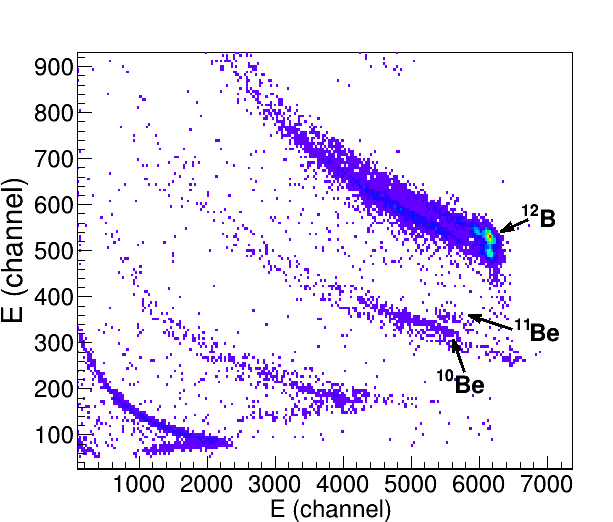
\includegraphics[width=1.0\columnwidth]{PIDf.png}\\
  \caption{The $\Delta E-E$ spectrum obtained using one of the recoil detector telescope with $^{12}$B incident on the (CD$_2)_n$ target. The data shown required a coincidence with a particle in the PSD array. The particle groups labeled $^{11}$Be($^{10}$Be), $^{12}$B are from neutron bound(unbound) states in $^{11}$Be and elastic scattering of $^{12}$B.}\label{protonE}
\end{figure}

The $^{11}$Be in Fig.~1 were used to discriminate the $^{12}$B$(d,^3$He) transition to the bound state of $^{11}$Be.  The $^{10}$Be ions with much wider energy distribution were generated from the transition to the  neutron-unbound states of $^{11}$Be.
With the energy loss of the escaping neutron, the average energy of $^{10}$Be is around 11 MeV lower than $^{11}$Be. Other possible sources of the $^{10}$Be ions in Fig.~1, like the $^{12}$B$(d,\alpha)^{10}$Be reaction, was mostly excluded. The present setup does not allow detection of the $^{12}$B$(d, \alpha)$ reaction to the bound state of $^{10}$Be. That is why we do not see the high-energy $^{10}$Be ions from the $^{12}$B$(d, \alpha)$ reaction channel.

\begin{figure}
  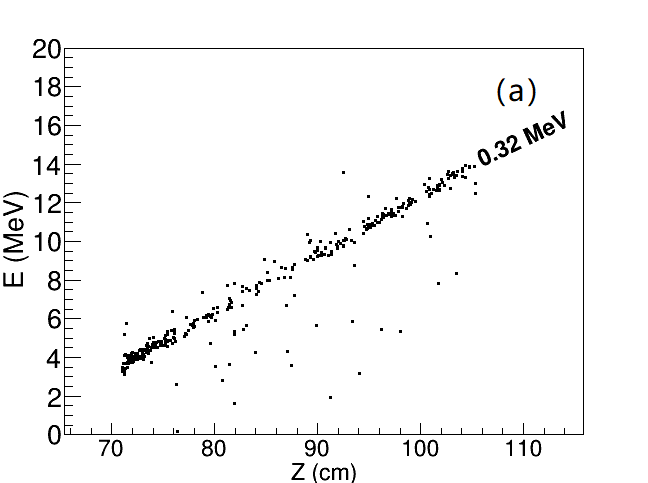
\includegraphics[width=1.0\columnwidth]{11BeEvZ.png}\\
    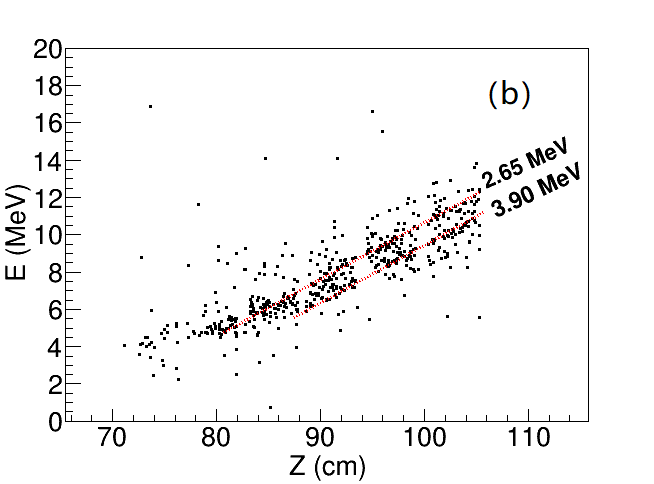
\includegraphics[width=1.0\columnwidth]{10BeEvZ.png}\\
  \caption{Measured proton energies ($E$) as a function of the distance from the target ($Z$) for the $^{12}$B$(d$,$^3$He)$^{11}$Be reaction in inverse kinematics at 12~MeV/u with a magnetic field strength of 2.3~T. The data shown required a coincidence with $^{11}$Be (a) and $^{10}$Be (b) in Fig.~1. Final states identified in $^{11}$Be are labelled by their corresponding excitation energy. The kinematics loci for different excited states appear as diagonal red-dotted lines. See details in the text.}\label{protonE}
\end{figure}

The the incident beam flux was monitored by the elastic scattering events on the PSD array.  Elastic scattering of $^{12}$B on deuterons was selected by requiring a 150-ns timing coincidence of a light particle on the PSD and a $^{12}$B ions identified in the recoil detectors (see Fig.~1). The deuterons traveling for four cyclotron periods were stopped on the PSDs and their numbers were used to determine the counts of incident particles timesing the target thickness. They were divided by the calculated cross sections combining with the acceptance of the experimental setup. The deuterons were measured at an energy of 3~MeV and at an c.m. angle of $\sim 23^{\circ}$, and their travelling periods were checked by the time of flight information. A variety of optical model potentials were used to calculate the elastic scattering cross sections. Uncertainties in the number of the $^{12}$B beam particles timesing the target thickness varies with an r.m.s of $\sim 30\%$, depending on different optical model parameters. A procedure for determining the absolute yield is described in Section IV.




\section{Results}

The events corresponding to the $^{12}$B$(d,^3$He)$^{11}$Be reaction to the bound or unbound states of $^{11}$Be were selected by requiring a $150-$ns timing coincidence between a light particle in the PSD array with a $^{11}$Be or $^{10}$Be ion discriminated in the recoil detectors. Most of the uncorrelated background was removed by using this timing coincidence. The energies of the light particles selected using this method are plotted in Fig.~2 versus the corresponding distance where the particles were detected by the PSD detectors. %The low energy events that were not in the ($d,^3$He) kinematic region were removed by a straight line in the spectrum of Fig.~2b.

For the present range covered by the PSD array, a clear isolated bound state in $^{11}$Be appears as a straight line in the plot (Fig.~2a). For the unbound states, their loci do not follow straight lines and different states merge at around $Z = 84$ cm. This is caused by the shallow orbitals of the $^3$He particles, which reached the PSD detectors at shorter distances than the ideal situation. This effect was observed in the previous $(d,^3$He) measurement~\cite{Bedoor2016} as well as the kinematics calculation. The red-dotted line in Fig.~2b represents the calculated kinematics of the ideal situation where the radius of the silicon array was assumed to be zero. Events were selected where the experimental kinematics loci follows the straight lines, and were used to obtain the excitation spectrum  as well as to evaluate the cross sections for the unbound states. The events obviously deviate from the straight kinematics lines were not used in the analysis.

\begin{figure}
  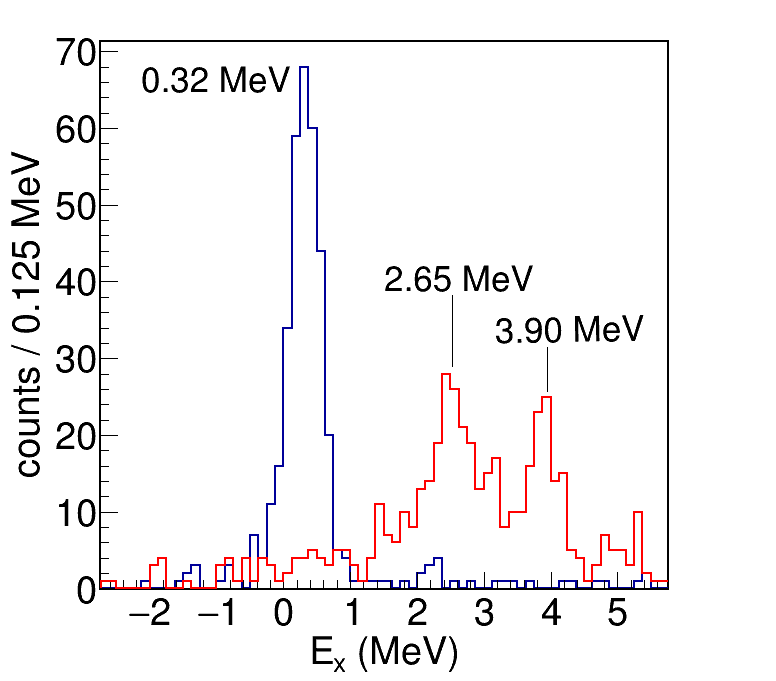
\includegraphics[width=0.8\columnwidth]{11BeEx.png}\\
  \caption{The excitation-energy spectrum of $^{11}$Be neutron bound (blue) and unbound (red) states determined from the data set as presented in Fig.~2(a) and (b) respectively. States clearly identified in the present work are labelled with their corresponding excitation energies.}\label{Ex}
\end{figure}

Excitation spectra for the $^{12}$B($d,^3$He) reactions were obtained from the projection of the data along the kinematic lines and the results are shown in Fig.~3, which presents data for both neutron-bound (blue) and unbound (red) states. The resolution for the excitation-energy spectrum of the bound state is around 560 keV (FWHM), dominated by the energy loss of the beam and $^3$He in the target as well as the angle straggling.   The measured widths of the unbound states are also contributed to by their intrinsic widths, which are 228(21) keV for the 2.65-MeV state~\cite{Liu1990} and 3.2(8) keV for the 3.90-MeV state~\cite{Fortune037302}. These widths are also compatible with the present spectrum given the appearance wider width of the 2.65-MeV state.

\linespread{1.3}
\begin{table}
\caption{\label{tab:table3} Spectroscopic factors $S$ for the $^{12}$B$(d,^3$He)$^{11}$Be reaction. The values are normalized such that the sum of $S$ over all transitions is 3.0. Relative uncertainties on $S$ are shown in parenthesis. Details on the uncertainties and the normalization factor is found in the text. }
\begin{ruledtabular}
  \begin{threeparttable}
\begin{tabular}{ccccc}
 \multicolumn{2}{c}{Literature}& &Present data &\\
\textrm{$E_x$ (MeV)}&
\textrm{$J_{\pi}$}&
\textrm{State}&
\textrm{$l$}&
\textrm{$S$}\\
\colrule\\
    0.00$^1$ & $1/2^+$  &    &  &  \\\\
    0.32 & $1/2^-$ & 0  & $l = 1$ & 0.56(12)  \\\\
   1.78$^1$ & $5/2^+$ &   &  &  \\\\
   2.65 & $3/2^-$ & 1  & $l = 1$ &  1.49(44)\\\\
   3.40$^1$ & $3/2^{(+,-)}$ &    &   &  \\\\
   3.89 & $5/2^-$ & \multirow{2}{*}{2}  & \multirow{2}{*}{$l = 1$} &\multirow{2}{*}{0.95(27)}  \\
   3.96 & $3/2^-$ &       \\\\
   5.26$^1$ & $5/2^-$ &   &   &  \\
   6.71$^1$ & $7/2^-$ &   &   &  \\
   \end{tabular}
\begin{tablenotes}
        \footnotesize
        \item[1] Not observed in the present measurement. See details in the text.
      \end{tablenotes}
    \end{threeparttable}
\end{ruledtabular}
\end{table}

Table I lists the states reported in the literature for $^{11}$Be~\cite{KELLEY2012}. Below the neutron-separation energy ($S_n=0.510$ MeV) of $^{11}$Be, the first excited state ($1/2^-$) at 320 keV was the most strongly populated state in the $^{12}$B$(d,^3$He) reaction. The unbound $3/2^-$ states at 2.654~MeV also presents as a strong transition in the present reaction. The next strongly populated state probably corresponds to the one or both of the states at 3.889~MeV and 3.955~MeV. The relative contribution of these two states is discussed in Section~VI.
The present resolution does not allow separation of the ground state and first excited state, which are just 320 keV apart. However, an upper limit of the ground state was estimated to be $8\%$ of the total events in the 320-keV peak, based on the standard deviation of $\chi^2$ method.
 Similarly, we cannot rule out some population of the 3.410-MeV state, which was assigned as $3/2^-$ or $3/2^+$ in the previous study. An upper limit for this states was drawn to be $10\%$ of the total events populated in the unbound states.

\section{Angular distributions}

\begin{figure}
  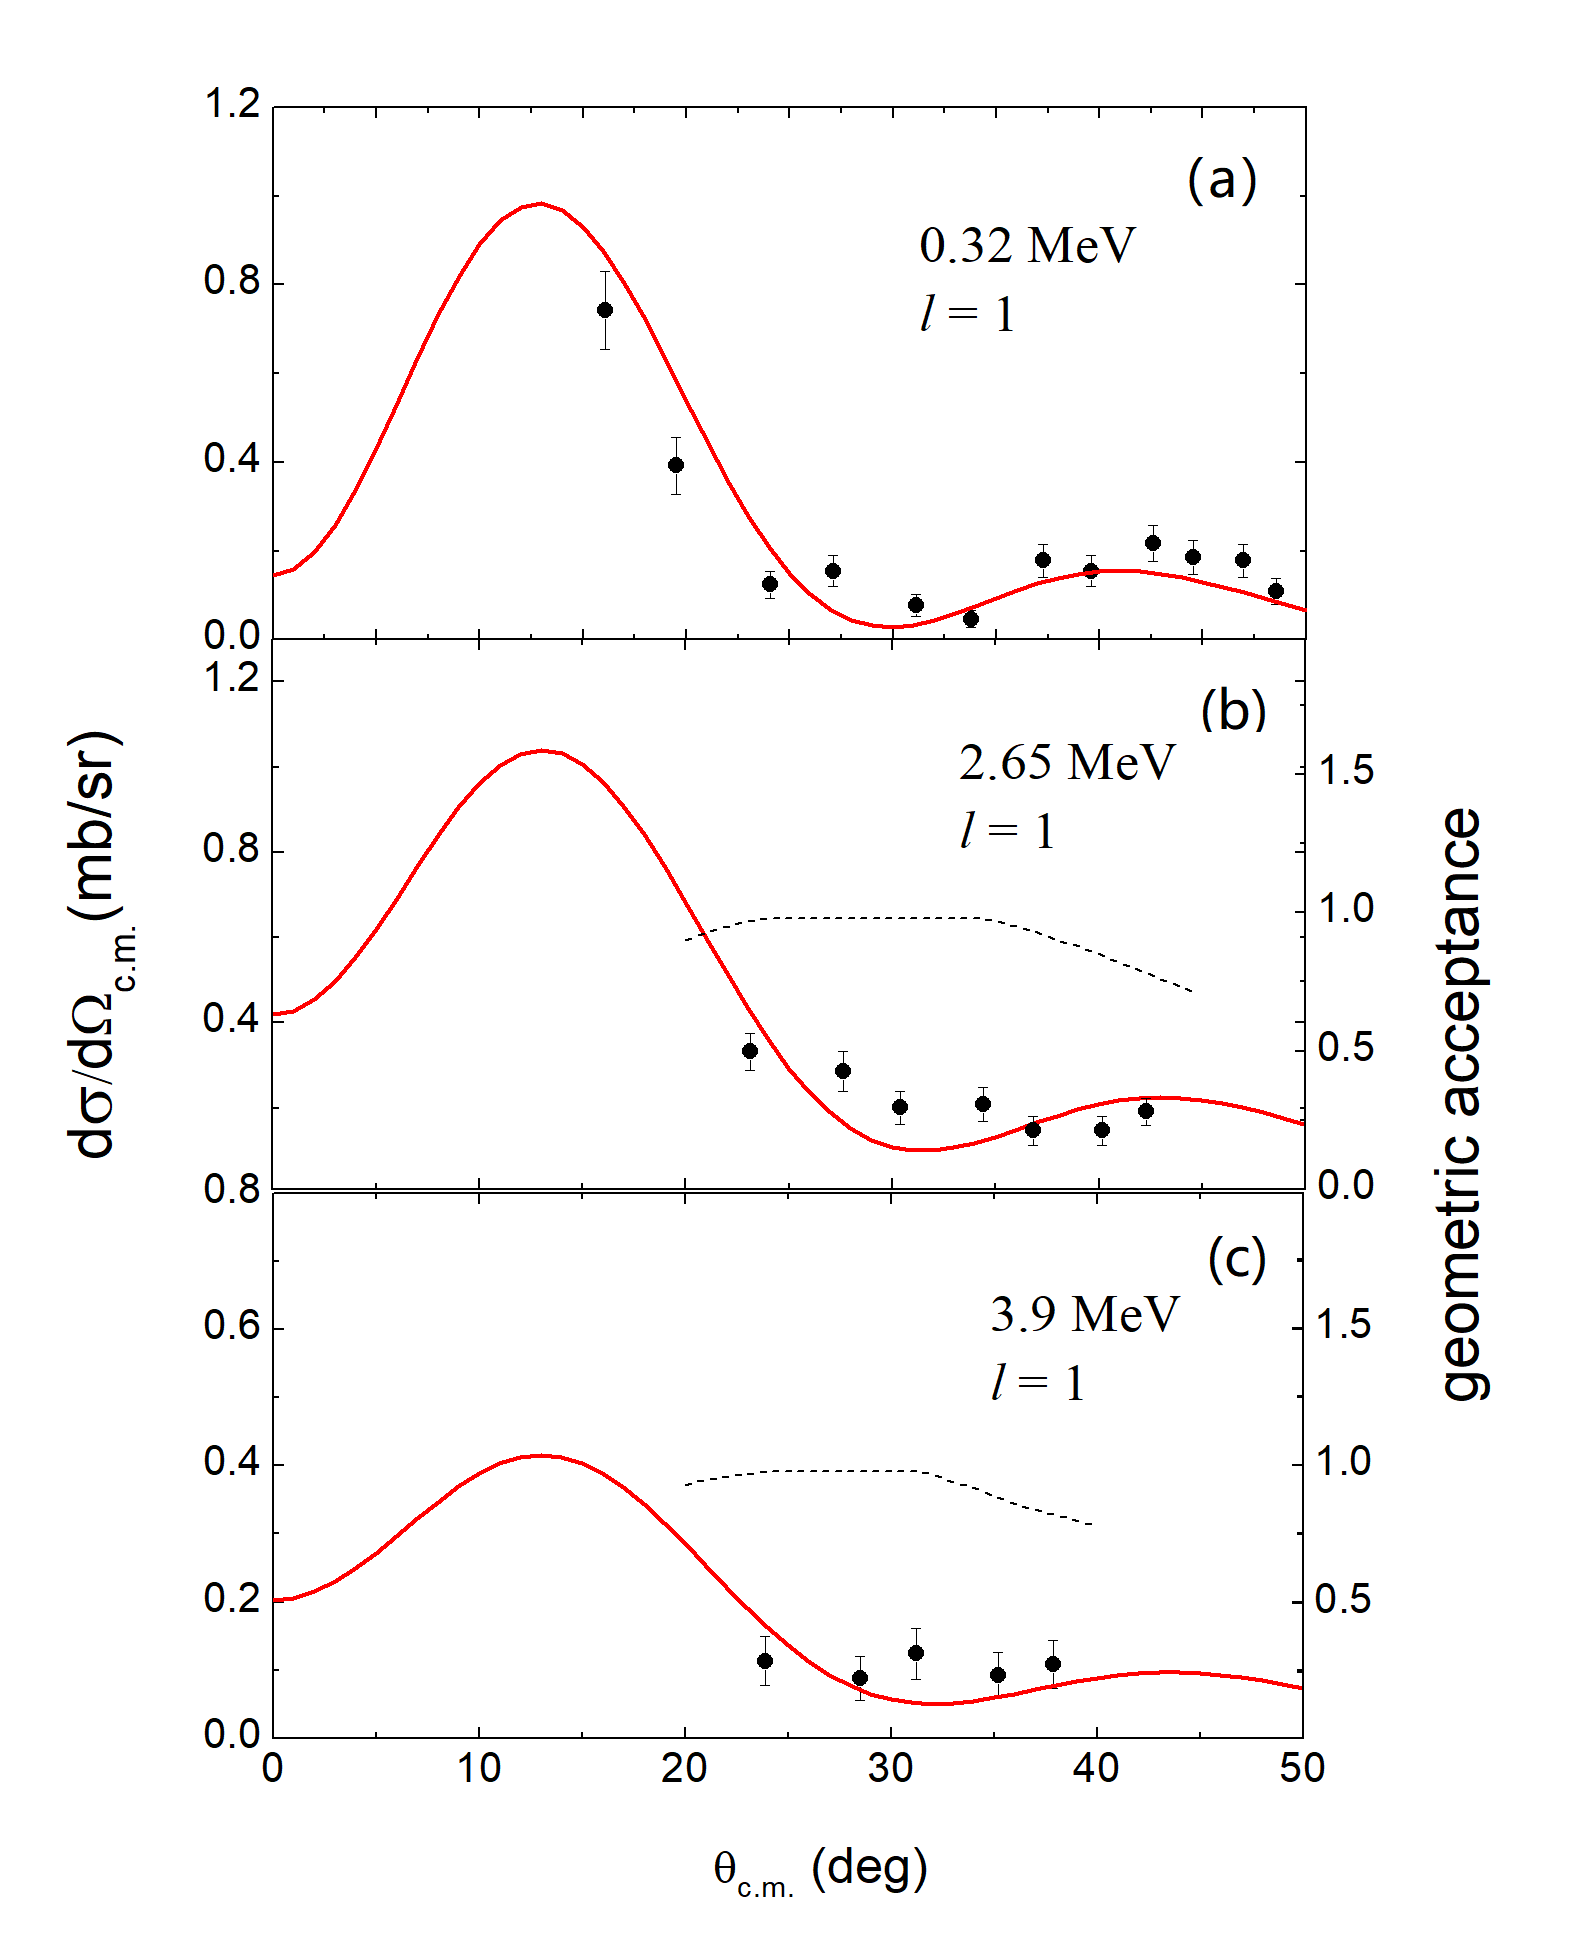
\includegraphics[width=1.0\columnwidth]{11BeCS.png}\\
  \caption{Experimental(black points) and calculated(solid lines) angular distribution for the (a)0.32-, (b)2.65- and (c)3.90-MeV transition in the $^{12}$B($d,^3$He)$^{11}$Be reaction. The curves represent DWBA calculations for $\ell=1$ transfer. Only statistical uncertainties are shown for the experimental data, and there is a systematic uncertainty of $\sim 30\%$ on the absolute cross section scale. The acceptance of the $^{10}$Be recoils for the neutron-unbound states of $^{11}$Be is plotted as dashed curves. }\label{Ex}
\end{figure}

The differential cross sections of each populated state of the $^{12}$B$(d,^3$He)$^{11}$Be reaction were deduced from the present data, using the Eq.~(4) in Ref.~\cite{Hoffman}. Every single PSD was either considered as a single center-of-mass angular bin or separated into two bins where the statistics allowed. The solid angle of each PSD detector is around 40 msr, and the center-of-mass angle ($\theta_{cm}$) for a bin was determined from the reaction kinematics and the properties of HELIOS within an uncertainty of $\sim 1^{\circ}$. It is noted that the acceptance of the recoiling $^{10}$Be generated from the unbound states of $^{11}$Be might decrease due to the breakup process. The acceptance of the $^{10}$Be ions generated from the isotopic decay of $^{11}$Be unbound states was calculated as a function of c.m. angles and plotted in Fig.~4. Within the range of the present data, the acceptance is mostly above 80$\%$, and was utilized to correct the cross sections.

As stated in the experimental part, the number of the incident beam timesing the the target thickness was estimated using the elastic scattering data on the PSD array. Combining this information with solid angles of the PSDs and the counts of each state, absolute cross sections were obtained from the present analysis, as shown in Fig.~4. Error bars in the figure are statistical only. There is a systematic uncertainty of around $30\%$ for the absolute cross sections, including the uncertainties from the determination of the beam particles, the target thickness and the cut on the PID spectrum. Most of the discussions in this paper focus on the relative $S$, so the uncertainty in the absolute cross sections has very little impact on the conclusions that are drawn based on the present work.

\section{DWBA calculations}

The spectroscopic factors were extracted from the differential cross sections through a DWBA analysis calculated using the program PTOLEMY~\cite{PTOLEMY}. The optical model parameter sets of An {\it et al.}~\cite{An} and Pang {\it et al.}~\cite{Pang} were used as the entrance and exit channels. The Argonne $V_{18}$~\cite{Wiringa} potential was used to define the deuteron bound-state wave function and a Woods-Saxon potential with central potential well parameters of $r_0 = 1.25$ fm and $a_0 = 0.65$ fm, and with spin-orbit parameters of $V_{so} = 6.0$ MeV, $r_{so} = 1.1$ fm, and $a_{so} = 0.65$ fm, was used to define the final bound state proton wave function. The depth of the Woods-Saxon potential well was adjusted to reproduce the correct binding energy of each of the final proton bound states in $^{11}$Be.

The calculated cross sections were normalized to the experimental angular distributions of each populated state using a standard $\chi^2$ method. The results are presented in Fig.~4. For the 320-keV state, the DWBA calculations with $l=1$ proton transfer reproduce the experimental angular distributions well. The 2.65-MeV and 3.89-MeV state data do not cover the most forward angular-distribution maximum due to the merged trajectories of these unbound states. Since the $l=1$ angular distribution of the 320-keV state is well reproduced by the DWBA calculation, we fit the angular distributions of the 2.65-MeV and 3.89-MeV state  for the experimental angular range, and larger uncertainties were determined for these states using various optical model potentials. The extracted spectroscopic factors $(S)$ and their corresponding strengths ($GS = S$) are listed in Table~I.


A variety of  optical model potentials~\cite{Han,An,Daehnick,Varner,Lohr,Pang,Liang2009} have been applied to the entrance and exit channels of the DWBA calculations to estimate uncertainties in $S$.  For the relative $S$, the uncertainties arise from the statistics, the fitting procedure, and variations in the DWBA analysis, with the sum of them being $\sim10\%$ for the 320-keV state and $\sim20\%$ for the 2.654-MeV and 3.889-MeV states.

\section{Normalization of the {\boldmath$GS$}}

In the present analysis, the observed $\pi0p_{3/2}$ strengths have been normalized to the occupancy of the orbital using the Macfarlane and French sum rule~\cite{Macfarlane}. In a simple single-particle picture, the sum of the $GS$ was normalized to 3, the occupancy of the $0p3/2$ and $0p1/2$ orbital, and the 320-keV, 2.654- and 3.899-MeV state were included in the normalization sum.  The $GS$ from higher negative excited states, like the 5.255-MeV state $(5/2^-)$, were assumed to be much smaller than these three states, which was supported by the shell model calculation (Section~IV). This normalization results in a normalization factor of 0.73(26), and the uncertainty was attributed from the absolute cross sections and different optical model potentials.

The entire procedure for the extraction and normalization of the $S$ was checked using the $^{11}$B$(d, ^3$He) data at 13.5 MeV/u taken with the same setup. We have obtained normalized spectroscopic factors of 0.61(6), 2.09(21) and 0.30(6) for the g.s., $2^+_1$ and $2^+_2$ state, using the same optical model parameters stated above. These results are consistent with those reported in Ref.~\cite{Schwinn1975}.

\section{Discussion}
There are three major peaks that were strongly populated in this reaction, corresponding to the $1/2^-$ at 0.32~MeV, the $3/2^-_1$ at 2.65~MeV, and the doublet at around 3.9~MeV.
The population of these states should correspond to removal of one $0p_{3/2}$ orbital proton from the ground state of $^{12}$B. The ground state of $^{12}$B is dominated by the $p$-shell neutron configuration with a very little $sd$-shell configuration~\cite{Mairle,Lind,LeeHY}. Further, one-proton removal  reaction on $^{13}$C~\cite{Mairle,Lind,Scott} indicates the $^{12}$B(g.s.) configuration is mostly $\pi(0p3/2)^{3}\nu(0p1/2)$. In principle, these strongly populated states are expected to be dominated by a configuration of $\pi(0p_{3/2})^2\nu(0p_{1/2})^1$.
The pair of protons in the $0p_{3/2}$ orbital could couple into $0^+$ and $2^+$. The states in $^{11}$Be with a $\pi(0p_{3/2})^2\nu(0p_{1/2})^1$ configuration can thus carry spin-parity of $1/2^-$, $3/2^-$ or $5/2^-$. In general, these negative-parity states are possibly dominated by two major neutron configurations, that is, the configuration within the $p$-shell orbitals ($0\hbar\omega$), and with two neutrons excited to the $sd$-shell ($2\hbar\omega$). The present reaction will selectively populate states with a dominant $0\hbar\omega$ configuration.

The first excited state at 0.32~MeV is expected to be dominated by the $p$-wave neutron configuration. This was confirmed by the one-neutron transfer reaction $^{10}$Be$(d,p)^{11}$Be~\cite{Schmitt}, which gives a large spectroscopic factor ($S=0.62(4)$) for the $l=1$ neutron component in this state. The first $3/2^-$ state at 2.65~MeV was previously seen in the $(t,p)$ reaction~\cite{Liu1990} and $\beta$-decay of $^{11}$Li~\cite{HIRAYAMA2005}, suggesting a normal $p$-shell neutron configuration. Our result confirmed these observations. The state at 3.889~MeV was previously assigned as $3/2^+$ in the $^9$Be$(t,p)^{11}$Be reaction measurement. However, the $\beta$-delayed decay study revised the spin-parity of this state as $5/2^-$. Regarding the likely strong population of this state in the present measurement, our results support the $5/2^-$ negative-parity assignment.

There are also some negative-parity states indicating dominant intruder configuration to the $sd$-shell orbitals. The $3/2^-_2$ state at 3.955~MeV should not be strongly populated in the present measurement, because it is suggested to be dominated by a configuration of $^9$Be$\otimes(sd^2)_{(2^+)}$ experimentally (see Table I in Ref.~\cite{Fortune2011}) as well as in the shell model calculation (see the next subsection). The situation is similar for the $5/2^-_2$ state at 5.26 MeV. %From the cluster model approach, these states are predicted to be the band member of $K^{\pi}=3/2^-$ with an $\alpha:3n:\alpha$ configuration~\cite{}.

In the following subsection, the effective-interaction shell-model, Nilsson-model, VMC and No-core shell-model will be discussed and compared with the experiments to clarify some of these ambiguities.

%For the positive-parity states, the g.s. ($1/2^+$) and the $5/2^+$ state at 1.78 MeV have dominant configurations of $^{10}$Be$\otimes1s_{1/2}$ and $^{10}$Be$\otimes1d_{5/2}$, respectively~\cite{}. There is also some $^{10}$Be$(2^+)$ core excitation component in the ground state.
%The 3.41-MeV state was assigned as $3/2^+$ according to the angular distribution of the inelastic scattering of $^{11}$Be on C target~\cite{Fukuda}. However, the same state was suggested to be $3/2^-$ in the $^{11}$Li $\beta$-decay measurement~\cite{HIRAYAMA2005} as well as the $^9$Be$(t,p)$ reaction~\cite{Liu1990}, although the authors showed some caution for certain spin-parity assignments. It is worth noting the relatively weak population of this state in the latter two measurements was possibly influenced by the multiple-step reactions.

\subsection{Shell model calculations}

\linespread{1.3}
\begin{table}
\caption{\label{tab:table3} Excitation energies $E_x$ and spectroscopic factors $S$ for the $^{12}$B$(d,^3$He)$^{11}$Be reaction calculated using the YSOX interaction~\cite{Yuan} and Nilsson model~\cite{Macchiavelli}. The values are normalized such that the sum of $S$ over all transitions is 3.0.}
\begin{ruledtabular}
  \begin{threeparttable}
\begin{tabular}{ccccccc}
 $^{11}$Be &\multicolumn{2}{c}{YSOX} &\multicolumn{2}{c}{WBP} & \multicolumn{2}{c}{Nilsson} \\%&\multicolumn{2}{c}{Present data} \\
\textrm{$J_{\pi}$}&
\textrm{$E_x$ (MeV)}&
\textrm{$S$}&
\textrm{$E_x$ (MeV)}&
\textrm{$S$}&
\textrm{$E_x$ (MeV)}&
\textrm{$S$}\\
\colrule
    $1/2^+$  &  0.00 & 0.003  &0.0 & 0.002&  &  \\%&  0.00 &  \\
    $1/2^-$ & 0.897 & 0.613  &-0.751 & 0.580& 0.125 & 1.5 \\%&  0.32 & 0.51\\
   $5/2^+$ & 1.355 & 0.004 & 0.853& 0.001& &  \\%&  1.78 &  \\
   $3/2^-_1$ & 3.091 & 1.481 & 0.947&0.909 & 2.375 & 1.2 \\%&  2.65 &  1.22\\
   $3/2^+$ & 3.994 &  $<0.001$ &3.232 & $<0.001$& &  \\%&  3.41  &\\
    $3/2^-_2$ &  4.636 & 0.265 & 3.090& 0.843& &  \\%&  3.96 &  \\
   $5/2^-_1$ & 4.918 & 0.633 & 2.845& 0.668& 3.569 & 0.3 \\%&  3.89 & 0.76\\
   $5/2^-_2$ &  6.105 & $<0.001$ & 5.495 & $<0.001$&  &  \\%&  5.26 & \\
   $7/2^-_1$ & 6.671 & $<0.001$& 6.496& $<0.001$& & \\
   $7/2^-_2$ & 9.365 &$<0.001$ & 7.219& $<0.001$& 8.875& \\
   \end{tabular}
    \end{threeparttable}
\end{ruledtabular}
\end{table}

\begin{table*}
\caption{\label{tab:table3} Shell-model occupation numbers for $^{12}$B and $^{11}$Be with the YSOX interaction.}
\begin{ruledtabular}
  \begin{threeparttable}
\begin{tabular}{cccccccccccc}
 & &\multicolumn{5}{c}{Protons}& \multicolumn{5}{c}{Neutrons}  \\
\textrm{$J_{\pi}$}&
\textrm{$E_x$ (MeV)}&
\textrm{$0p_{3/2}$}&
\textrm{$0p_{1/2}$}&
\textrm{$0d_{5/2}$}&
\textrm{$0d_{3/2}$}&
\textrm{$0s_{1/2}$}&
\textrm{$0p_{3/2}$}&
\textrm{$0p_{1/2}$}&
\textrm{$0d_{5/2}$}&
\textrm{$0d_{3/2}$}&
\textrm{$0s_{1/2}$}\\
\colrule
    $1^+$ & $^{12}$B g.s. & 2.701 & 0.193 & 0.04 & 0.052 & 0.014 & 3.733 & 1.117 & 0.071 & 0.061 & 0.018\\
    $1/2^+$ & 0.00 & 1.747 & 0.222 & 0.009 &  0.017 & 0.005 & 3.459 & 0.483 & 0.227 & 0.04 & 0.792\\
    $1/2^-_1$ & 0.897 & 1.8 & 0.162 & 0.009 &  0.025 & 0.005 & 3.85 & 1.05 & 0.05 & 0.042 & 0.009\\
   $5/2^+$ & 1.355 & 1.71 & 0.259 & 0.01 &  0.017 & 0.004 & 3.442 & 0.502 & 0.859 & 0.061 & 0.137 \\
   $3/2^-_1$ & 3.091 & 1.797 & 0.148 & 0.015 & 0.03 &  0.009 & 3.374 & 1.138 & 0.294 & 0.061 & 0.133 \\
   $3/2^+$ & 3.994 &  1.697 & 0.269 & 0.012 & 0.018 & 0.005 & 3.388 & 0.552 & 0.244 & 0.208 & 0.608 \\
   $3/2^-_2$ &  4.636 & 1.658 & 0.314 & 0.01 & 0.015  & 0.004 & 2.935 & 0.545 & 0.718 & 0.125 & 0.677\\
   $5/2^-_1$ & 4.918 & 1.769 & 0.179 & 0.019 &  0.026 & 0.007 & 3.788 & 1.027 & 0.095 & 0.055 & 0.035 \\
   $5/2^-_2$ &  6.105 & 1.624 & 0.356 & 0.006 & 0.011  & 0.003 & 2.675 & 0.41 & 1.032 & 0.176 & 0.792\\
   $7/2^-_1$ & 6.671 & 1.629 & 0.343	& 0.008 & 0.016 &	0.004 & 2.614 & 0.418 & 1.145 & 0.233 &	0.59 \\
    $7/2^-_2$ & 9.365 &1.884 & 0.041	& 0.029 & 0.036	& 0.01 & 2.919 & 1.693	& 0.063 &	0.239 &	0.086\\

   \end{tabular}
%\begin{tablenotes}
        %\footnotesize
        %\item[1] Not observed in the present measurement. See details in the text.
%        \item[2] The states were not resolved in the measurement due to the small strengths. The value was estimated using existing experimental results.
%        \item[3] Obtained using average of the experimental results in the table.
%       \item[4] Root Mean Square (RMS) values of the deviation of the experimental results from the average values.
      %\end{tablenotes}
    \end{threeparttable}
\end{ruledtabular}
\end{table*}

We have performed the shell model calculations for $^{12}$B and $^{11}$Be with the WBP interaction and recently developed YSOX interaction~\cite{Yuan}. The calculations assume $^4$He as an inert core, and particles could occupy the $0p_{1/2}$, $0p_{3/2}$, $1s_{1/2}$, $0d_{5/2}$ and $0d_{3/2}$ orbitals. The calculated $^{11}$Be excitation energies and corresponding spectroscopic factors $S$  are given in Table~II. Further information about the occupation number of each orbital can be found in Table~III.
% The WBP interaction was constructed in the $(0-1)\hbar\omega$ model space, which means that 0-1 nucleons are allowed to be excited to the $sd-$shell. The $\langle pp|V|sdsd \rangle$ matrix element represents the interaction between $(0-1)\hbar\omega$ and $(2-3)\hbar\omega$ states have not been included in the fitting.
The YSOX interaction reproduces well the ground-state energies, energy levels, electric quadrupole properties, and spin properties for most nuclei in the full $psd$ model space including $(0-3)\hbar\omega$  excitations~\cite{Yuan}. The level order of the ground state and first excited state is inverted in the calculation using the WBP interaction while it is well reproduced using the YSOX interaction. We will focus the discussion with calculations using the YSOX interaction.

According to the calculations using the YSOX interaction, the spectroscopic factors to the $1/2^+$ and $5/2^+$ states can be neglected in the $^{12}$B$(d,^3$He)$^{11}$Be reaction. The $1/2^-$, $3/2^-_1$ and $5/2^-_1$ states have large overlaps with the $^{12}$B g.s., corresponding to the experimentally observed states at 320~keV, 2.654~MeV, and 3.899~MeV. These states have a configuration with one particle in $0p_{1/2}$ orbital, with very little excitation to the $sd$ shell, consistent with our previous discussion. The calculated $S$ (Table~III) of the former two states are in reasonable agreement with the experimental values.
The $3/2^-_2$ state in the calculation probably corresponds to the 3.955-MeV state, and it is dominated by a $2\hbar\omega$ configuration, which has a very small overlap with the $^{12}$B g.s.
  The $S$ of the $3/2^-_2$ and the $5/2^-_1$ state are added and compared with the experimental spectroscopic factor of the doublet around 3.9~MeV, showing reasonable agreement. It worth noting that the experimentally observed events at around 3.9~MeV should be dominated by the 3.899-MeV state, with a smaller contribution from the 3.955-MeV state due to the configuration mixing of the 0$\hbar\omega$ excitation.

   The maximum angular momentum that can be obtained within the $p$-shell orbitals is $7/2^-$. However, the present reaction will not populate it because of the $l=1$ transferred angular momentum. We also listed the shell model calculation for the first two $7/2^-$ states in Table~II and III for comparison.

 There is another $5/2^-$ state at around 6~MeV in the calculation, with a $2\hbar\omega$ configuration, which probably corresponds to the previously observed 5.255-MeV state in the $^9$Be$(t,p)$ reaction~\cite{Liu1990}. This state could  not be observed in the present measurement due to the acceptance of the setup. However, the calculated spectroscopic factor for this state is much smaller than the $5/2^-_1$ state or the $3/2^-_1$ states, indicating the $p$-wave strength observed in this measurement could account for most of the proton removal strengths in the $0p_{3/2}$ orbital, and it is reasonable to normalize the sum of them to the occupancy of the $0p_{3/2}$ orbital in the $^{12}$B g.s. For another, there is no strong indication of another low-lying $3/2^-$ state with $2\hbar\omega$ configuration in the calculation, in contrast to the previous suggestion for the 3.410-MeV state in the $(t,p)$ reaction.


\subsection{Nilsson model calculations}

\begin{figure}
  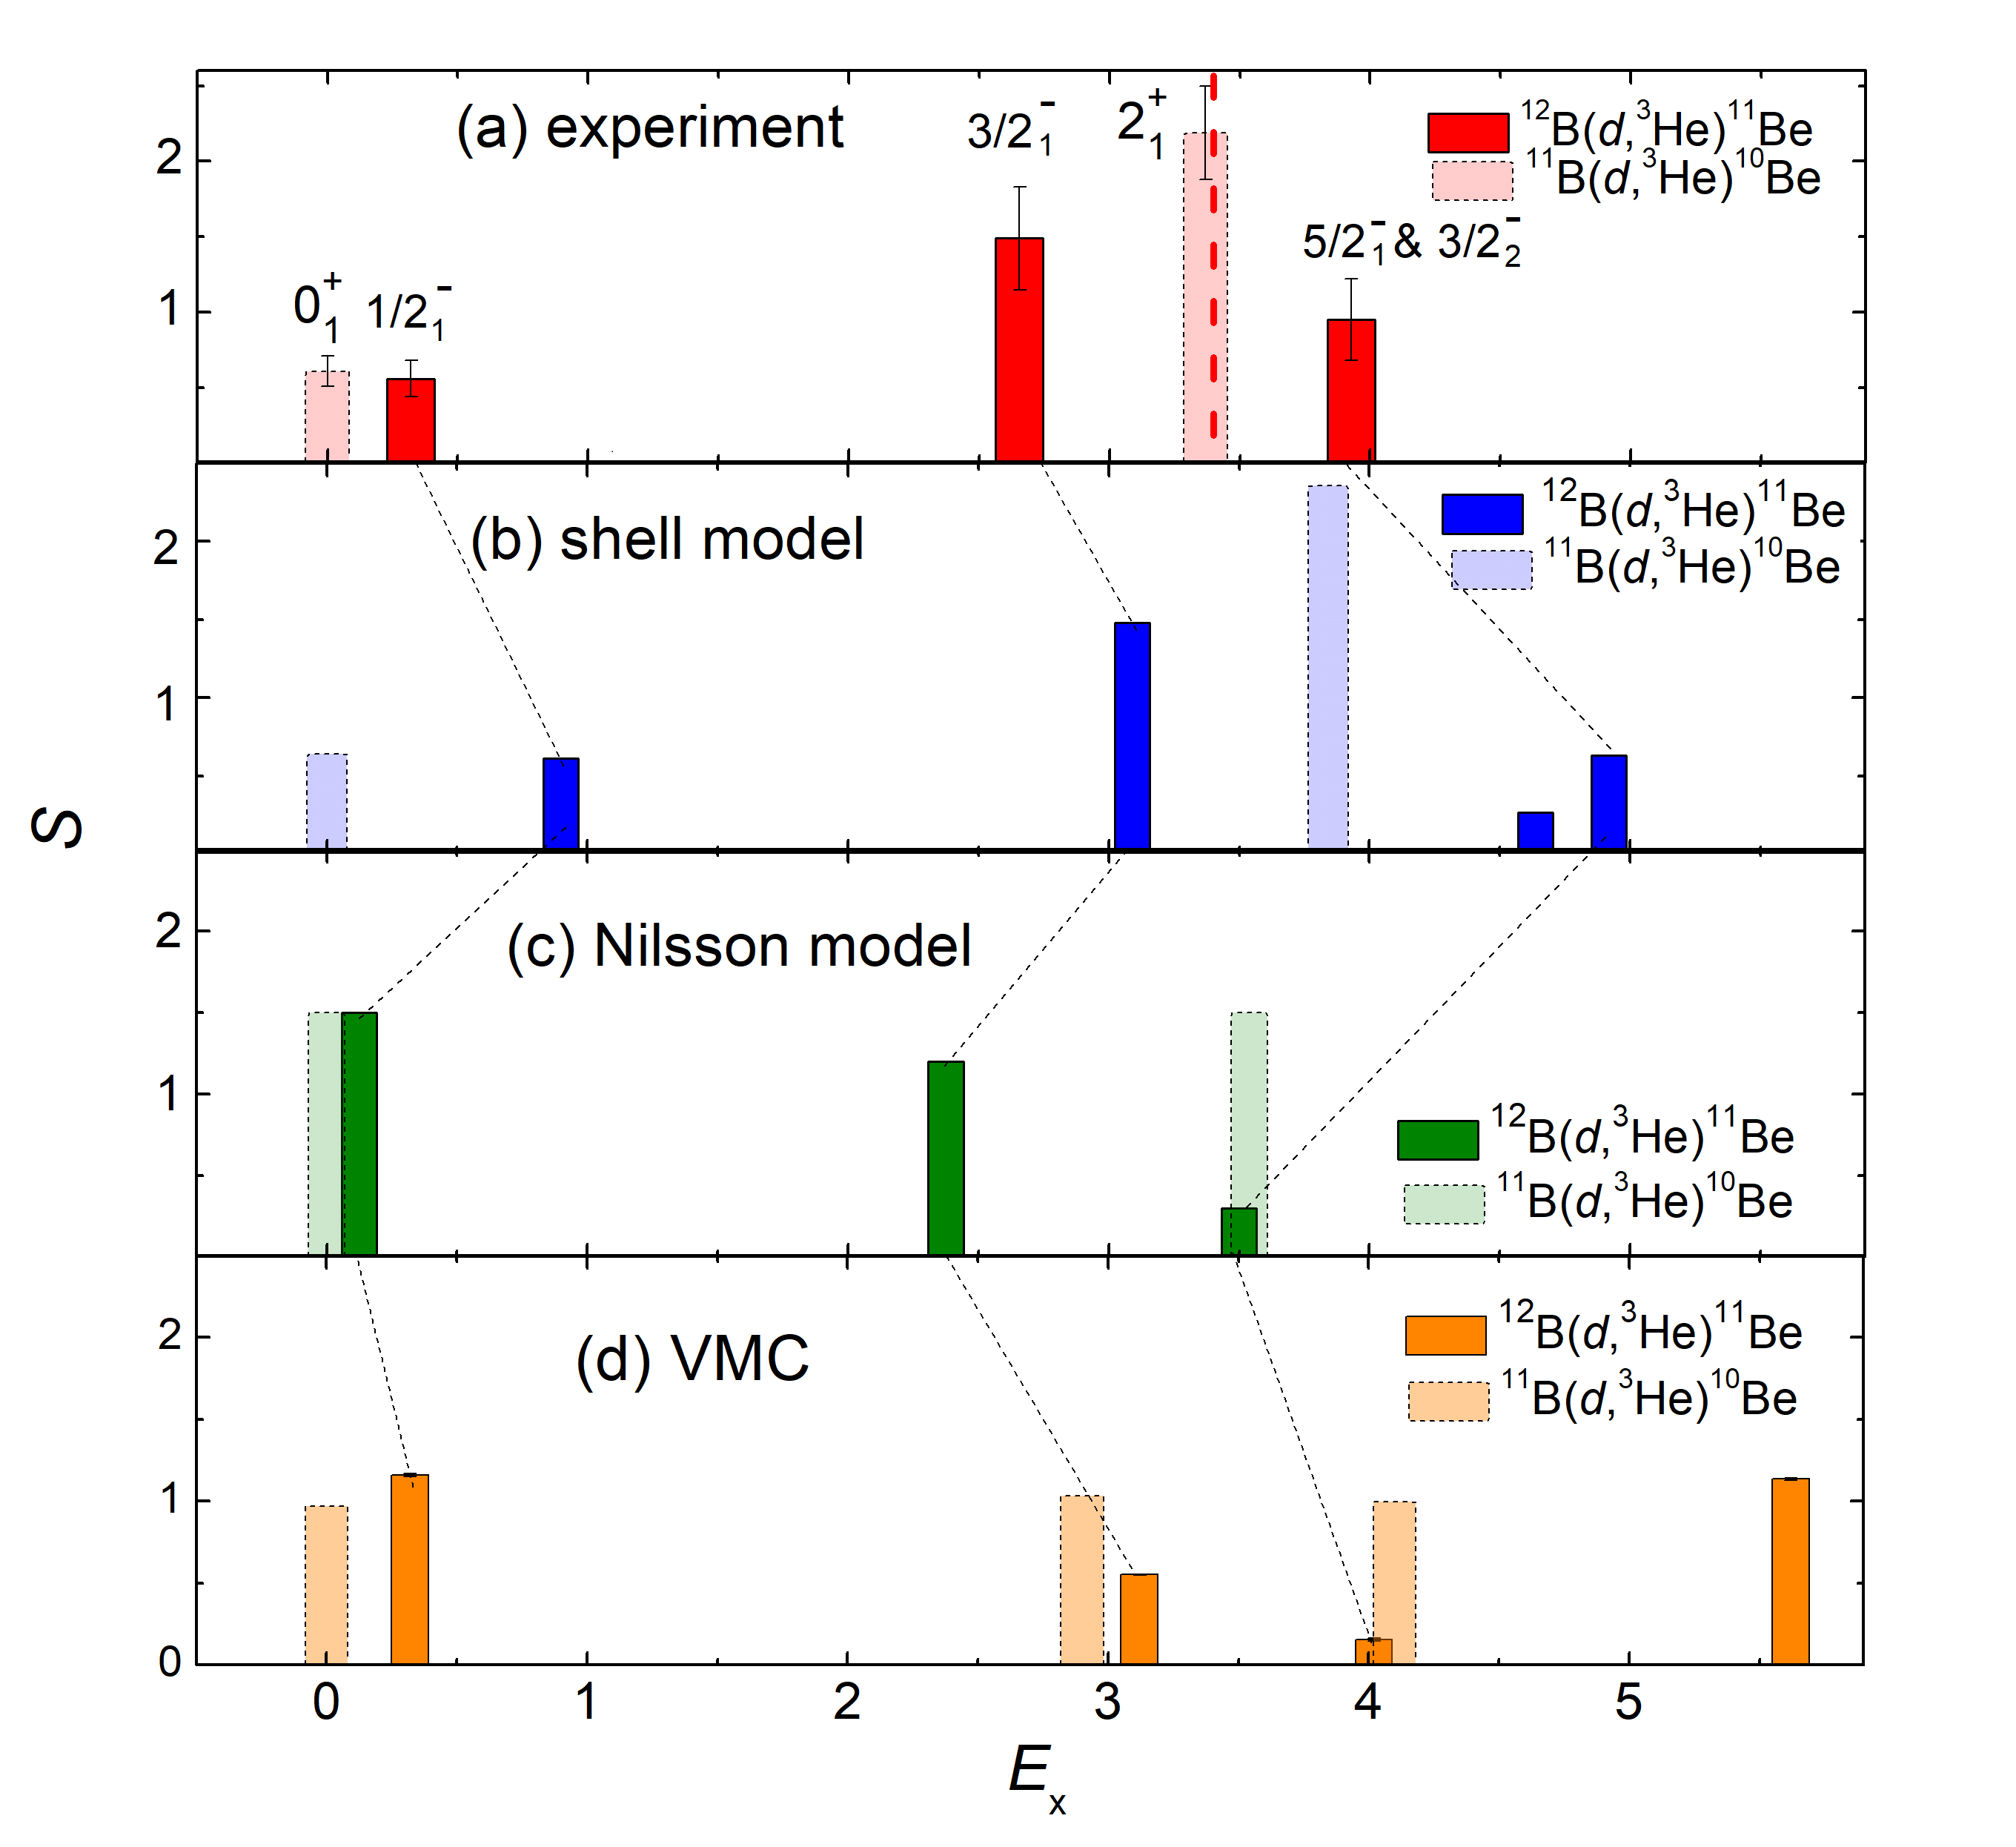
\includegraphics[width=1.1\columnwidth]{11Be_compare.png}\\
  \caption{The experimental (a) and calculated (b,c,d) excitation energies and spectroscopic factors of the $1/2^-_1$, $3/2^-_1$, $5/2^-_1$ states of $^{11}$Be $^{12}$B($d,^3$He)$^{11}$Be reaction and  $0_1^+$ and $2_1^+$ state of $^{10}$Be in the $^{11}$B($d,^3$He)$^{10}$Be reaction. (b), (c) and (d) were calculated using shell model with YSOX interaction, Nilsson model and VMC method, respectively. The error bars for the experimental values are just for relative $S$. The dashed line in (a) is the $2j+1$ weighted energy centroid of $3/2^-_1$ and $5/2^-_1$ states in $^{11}$Be. %Energies and spectroscopic factors for $$transitions from theory and experiment
  }\label{Ex}
\end{figure}

Here we understand the structure of the neutron-rich Be isotopes within the Nilsson model to study their collective degree of freedom. Within this framework, the $1/2^-_1$, $3/2^-_1$ and $5/2^-_1$ are band members of $K^{\pi}=1/2^-$, and using ~\cite{Bohr}
\begin{equation}\label{Ex}
 \begin{split}
E_x(J) = \frac{{\hbar}^2} {2\Theta} \cdot [J(J+1)+a\cdot(-1)^{J+1/2}\cdot\\(J+1/2)]
+E_0,
 \end{split}
\end{equation}
their excitation energies were calculated with the band parameter $b = \hbar/2\Theta =0.5$ MeV and the Coriolis decoupling parameter $a=0.5$. This band is expected to be terminated by the $7/2^-$ state with all the angular momentum of the valence nucleons aligned. It appears that the second $7/2^-$ state in Table II belongs to this band due to its dominant configuration within the $p$-shell. The first $7/2^-$ probably corresponds to the member of the long $2\alpha$-cluster band, which were understood as dominant by 2$\hbar\omega$ configurations in the shell-model picture. %
 Within the Nilsson scheme, the $Z = 5$ proton is expected to occupy the $3/2[101]$ level and the g.s. of $^{12}$B belong to band with $K^{\pi}=1^-$. Since the level parentage is attributed only to the $0p_{3/2}$ orbit, the spectroscopic factors depend only on the Clebsch-Gordan coefficients according to Eq.~3 of Ref.~\cite{Macchiavelli}, and we predict the $S$ as listed in Table~II, which were also normalized to the occupancy of the orbitals.

\subsection{VMC calculation}%{\boldmath$ab$-$initio$} calculations}

(to be continued)

\subsection{No-core shell-model calculation}%{\boldmath$ab$-$initio$} calculations}

(to be continued)


\subsection{Comparisons}

 The $^{11}$B($d,^3$He)$^{10}$Be reaction also serves as another testing ground for the Nilsson model. Information could be obtained from previous data as well as the stable beam data in the present experiment. Both measurement agree on spectroscopic factors of around 0.6(6) and 2.1(21) for the $0^+_1$ and $2^+_1$ states.  In order to further understand the experimental results, we also compare the experimental spectroscopic factors of the $^{11}$B($d,^3$He)$^{10}$Be to the calculated ones of shell model using the YOSX interaction as well as Nillson model.
Fig.~5 represents these calculated spectroscopic factors and excitation energies in comparison with the experiments, for the $1/2^-_1$, $3/2^-_1$, $5/2^-_1$ states of $^{11}$Be in the $^{12}$B($d,^3$He)$^{11}$Be reaction and $0_1^+$ and $2_1^+$ states of $^{10}$Be in the $^{11}$B($d,^3$He)$^{10}$Be reaction. Excitation energies of the $2^+$ state of $^{10}$Be in the Nilsson model was calculated using $b=0.59$. Although the Nilsson model reproduces their energies, the spectroscopic factors are underestimated for the $3/2^-_1$, $5/2^-_1$ states in $^{11}$Be and $2_1^+$ state in $^{10}$Be.
%One possible explanation for the failure of the Nilsson-model calculations is the very different deformation in the Be and B isotopes. Be isotopes are well-known for the underlying $\alpha$-cluster structure while there is no such indications in the B isotopes.

Experimental and theoretical studies hinted on the possible existence of the $N=6$ shell closures in $^8$He~\cite{Skaza} and $^{14}$O~\cite{ANGELI,Otsuka2001}. More recently, various sides of evidences for the $Z=6$ shell closure in $^{13-20}$C has been reported~\cite{Tran2018}. If we assume that $N=6$ is a subshell, the $1/2^-_1$, $3/2^-_1$ and $5/2^-_1$ states could be viewed as composed of one neutron in $0p_{1/2}$ orbital outside the $^{10}$Be($0^+$) or $^{10}$Be($2^+$) core. The $2j+1$ weighted energy centroid of $3/2^-_1$ and $5/2^-_1$ states (shown as dashed red line in Fig.~5) compared to $1/2^-_1$ state in $^{11}$Be is close to the energy difference of $2^+_1$ and $0^+_1$ states in $^{10}$Be. Further, the spectroscopic factors of $1/2^-_1$ state and the sum of $3/2^-_1$ and $5/2^-_1$ states are close to the values of $0^+_1$ and $2^+_1$ states for the $^{11,12}$B$(d,^3$He) transition, respectively (see Fig.~5). The situation is similar in the shell model calculations using YSOX interaction. Spectroscopic study of the negative-parity states populated in the proton removal reactions on $^{11,12}$B shows a consistent picture, with the valence neutron in  the $0p_{1/2}$ orbital coupling to the $^{10}$Be core.


%\begin{figure}
 % 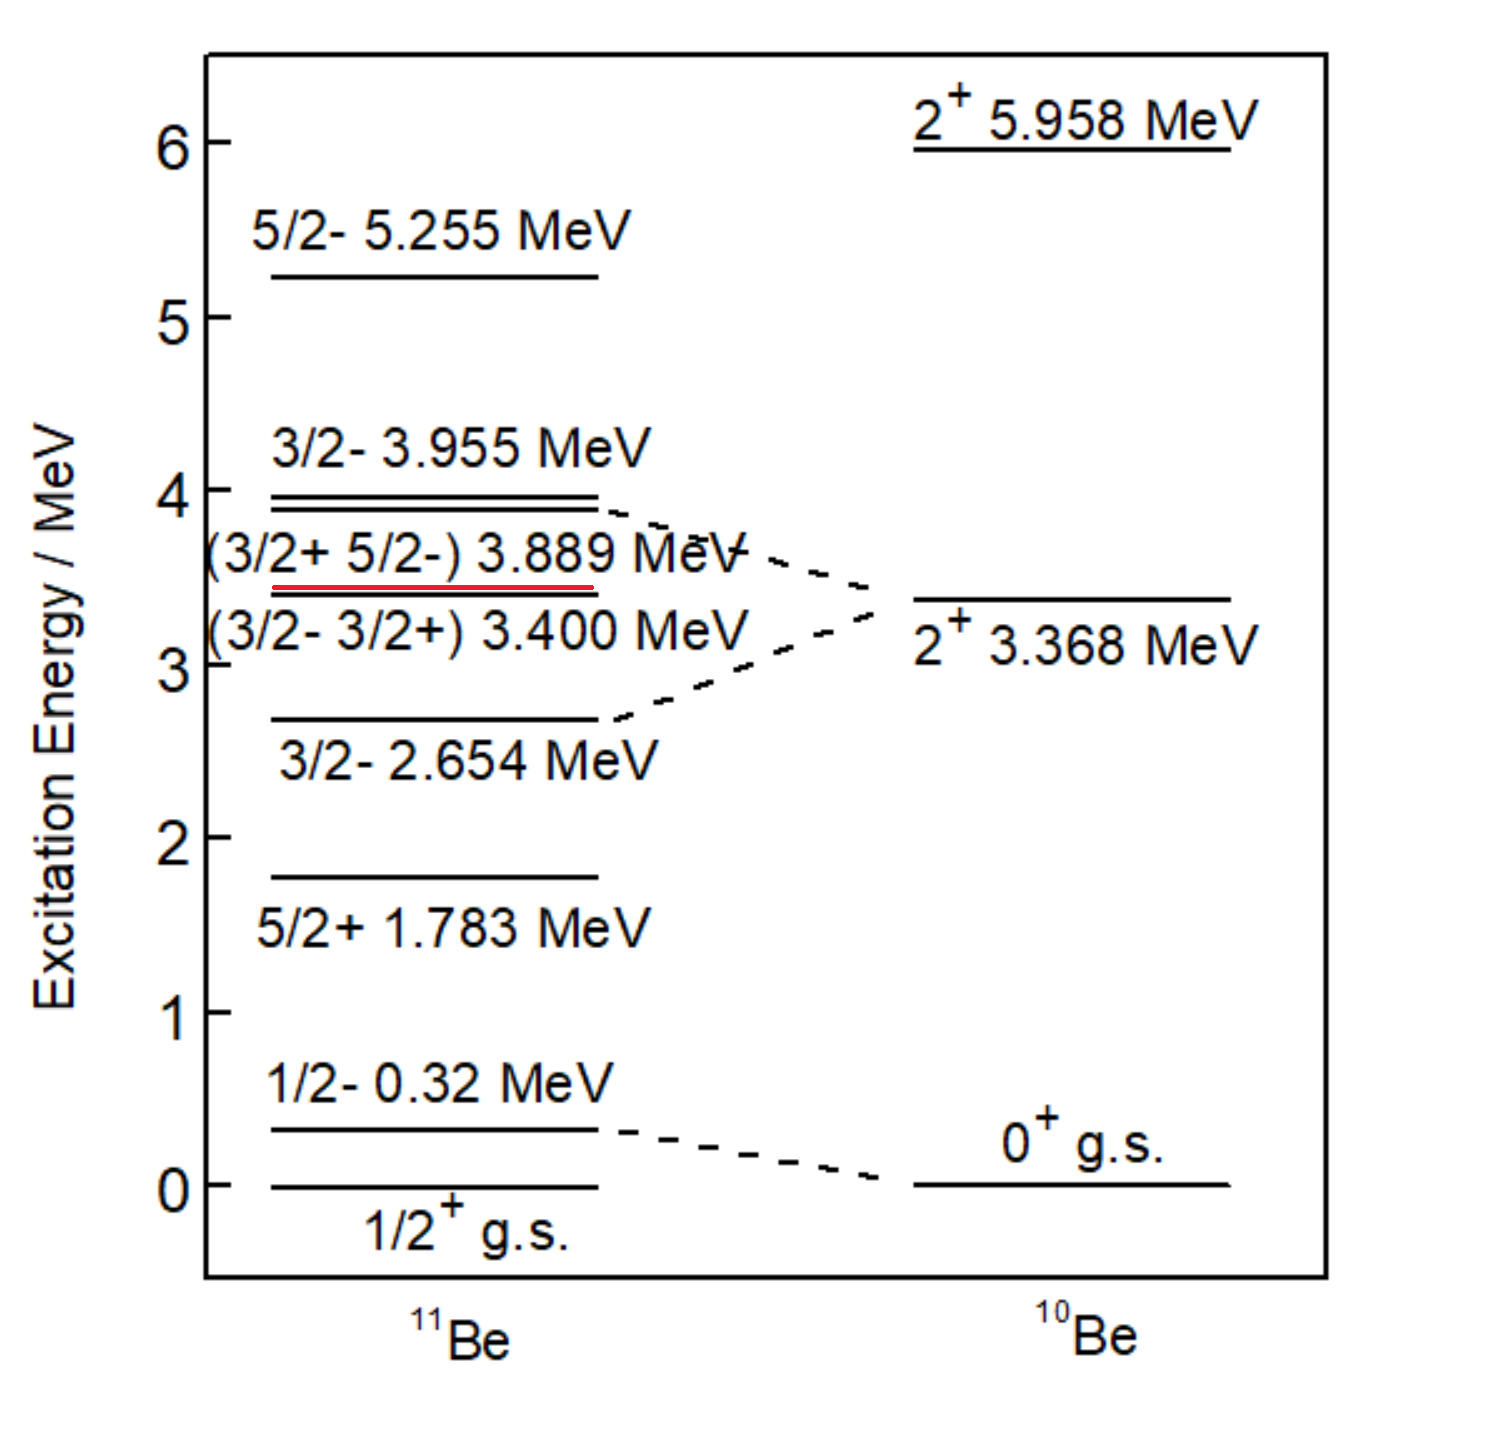
\includegraphics[width=1.0\columnwidth]{10Be_11Be.png}\\
  %\caption{The excitation energy of the first $2^+$ state, compared to the energy difference of the centroid (red line) of $3/2^-_1$ and $5/2^-_1$ states relative to the $1/2^-$ state in $^{11}$Be. Note that the excitation energy of the $2^+$ state in (c) is taken from the experimental values.%The red line represents the energy centroid of the $3/2^-_1$ and $5/2^-_1$ states.
  %}\label{Ex}
%\end{figure}



\section{Summary}




\begin{acknowledgments}

The authors would like to acknowledge the hard work of the support and operations staff at ATLAS. This research used resources of Argonne National Laboratory's ATLAS facility, which is a Department of Energy Office of Science User Facility. This material is based upon work supported by the U.S. Department of Energy, Office of Science, Office of Nuclear Physics, under Contract No. DE-AC02-06CH11357 (ANL) and Grant No. DE-FG02-96ER40978 (LSU).  J.~C. acknowledges partial support by the FRIB-CSC Fellowship under Grand No.201600090345.

\end{acknowledgments}

\bibliography{12Bdh}% Produces the bibliography via BibTeX.

\end{document}
%
% ****** End of file apssamp.tex ******
